\chapter{Implementazione}
In questo capitolo mostreremo come sono stati implementati i servizi REST per i requisiti funzionali elencati nella tabella \ref{tab:req:fun}.
Vedremo quindi per ogni requisito quali API sono state create, come sono state documentate ed il codice che abbiamo implementato per ciascuna di esse.

\section{FUN-01}
Per implementare il primo requisito funzionale che prevede l'utilizzo dei propri dispositivi con l'app, abbiamo creato quattro servizi.
Il primo, /device/output/, serve per richiedere l'array dei propri dispositivi.
Qui di seguito il codice relativo alla rotta:
\begin{lstlisting}[caption={/webserver/app/routes/device.js output}, style=javaScriptCode]
  router.get('/output', function(req, res) {
    if(req.user.block) {
      res.status(401).send({'msg':'Authentication required'});
    } else {
      Device.find({_GPIO:{$ne: null}, permission:{$gte: req.user.permission}, 
                                                      io:"output"})
        .populate('_Beacon _GPIO')
        .exec(function (err, devices) {
          if(err) {
            debugger;
            res.status(500).send({msg: err.errmsg});
          } else if(devices && devices.length>0) {
            res.status(200).send(devices);
          } else {
            res.status(200).send([]);
          }
      });
    }
  });
\end{lstlisting}
Il server controlla se l'utente che ha richiesto la lista dei dispositivi abbia effettuato il login e non sia stato bloccato.
Se non ha i permessi risponderà con un 401, altrimenti ricercherà tra tutti i dispositivi quelli che hanno un GPIO configurato e a cui può accedere l'utente. 
Così come descritto nella figura \ref{fig:device:output}\footnote{La documentazione è state scritta con swagger. Per consultarla, una volta avviato il backend, basta visitare la pagina \url{http://localhost:8000/swagger-ui/dist/} }. 

\begin{figure}[h]
\centering
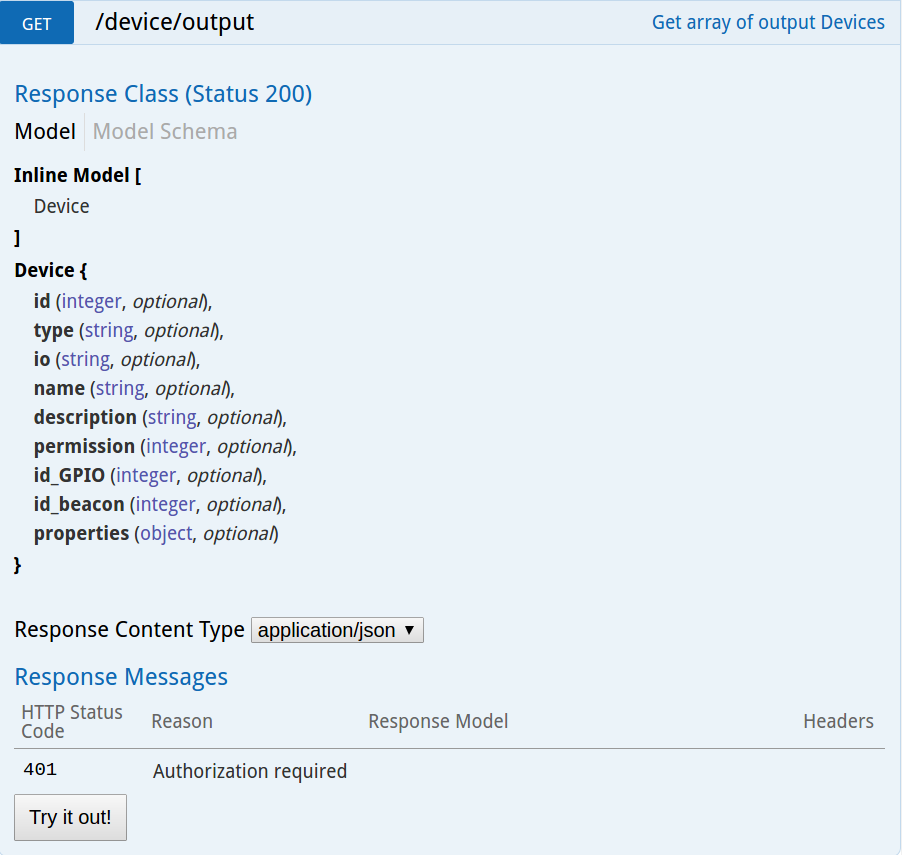
\includegraphics[width=1\textwidth]{API/device_output.png} 
\caption{Documentazione /device/output}
\label{fig:device:output}
\end{figure}

Le altre tre sono molto simili e sono /device/on, /device/off e /device/push.
Queste permettono di gestire i GPIO associati ai dispositivi settandoli rispettivamente a true, false e di inviare un impulso.

\newpage
Per queste tre rotte vedremo il codice solo della prima perché sono molto simili tra loro.
\begin{lstlisting}[caption={/webserver/app/routes/device.js on}, style=javaScriptCode]
  //need permission to do an action
  router.put('/:id/on', function(req, res) {
    if(req.user.block) {
      res.status(401).send({'msg':'Authentication required'});
    } else {
      Device.findById(req.params.id)
        .populate('_GPIO')
        .exec(function(err, device) {
          if(err) {
            debugger;
            res.status(500).send({msg: err.errmsg});
          } else if(device) {
            GPIO.update({_id: device._GPIO}, {value: true}, {}, 
                                         function (err, ok) {
              if(err) {
                res.status(500).send({msg: err.errmsg});
              } else {
                pin.setPin(device._GPIO.GPIO, true, function(err) {
                  if (err) {
                    res.status(500).send('Oops, Something went wrong! '
                                                      + err);
                  } else {
                    io.emit('update:device');
                    io.emit('update:gpio');
                    res.status(200).send({'msg':'ok'});
                  }
                }, environment);
              }
            });
          } else {
            res.status(404).send([]);
          }
        });
      }
    });
\end{lstlisting}
Quello che salta all'occhio sono le due funzioni pin.setPin e io.emit.
La funzione pin.setPin permette di settare il GPIO del RaspberryPI.
Mentre io.emit serve per inviare una notifica push a tutti i client connessi che li avvisa che i dati dei dispositivi e dei GPIO sono stati aggiornati, sarà poi il client a decidere se è il caso di aggiornarli oppure no.  

Come passare i parametri e come risponde il server è descritto nella documentazione.
\begin{figure}[h]
\centering
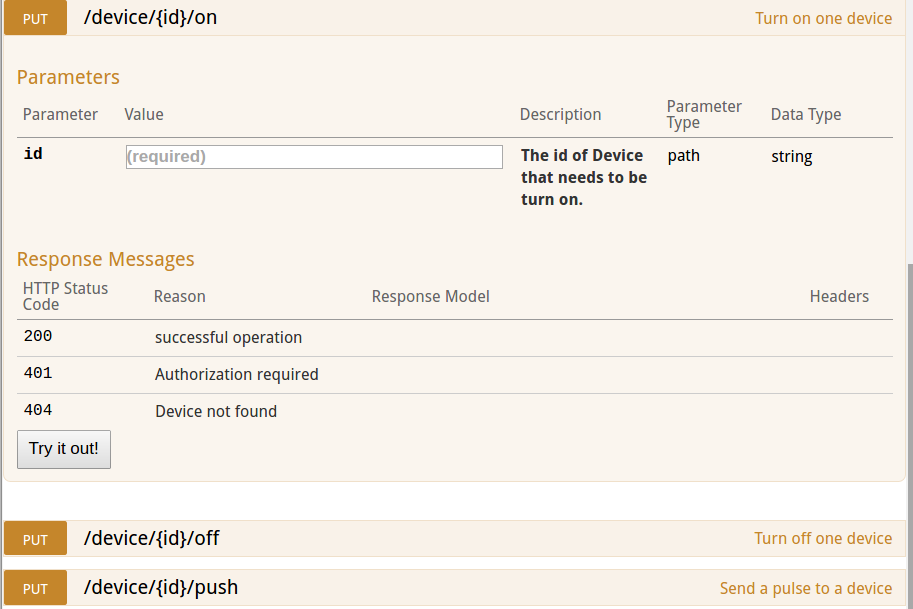
\includegraphics[width=1\textwidth]{API/device_on.png} 
\caption{Documentazione /device/{id}/on}
\label{fig:device:on}
\end{figure}

Nella figura \ref{fig:device:on} si vedono solamente i parametri e i messaggi di risposta della prima, ma sono gli stessi anche per le altre due.

\section{FUN-02}
Il secondo requisito parla di fornire agli utenti dell'app di effettuare il login e la registrazione.
Lato backend si è tradotto in tre API.
Una richiesta in post per il login.
Una richiesta in post per la registrazione e un'ultima richiesta per verificare che l'username scelto dall'utente sia disponibile in quanto deve essere univoco. 

\begin{lstlisting}[caption={/webserver/app/routes/user.js login}, style=javaScriptCode]
  router.post('/login', function(req, res) {
    if(req.body.username && req.body.password) {
      User.findOne({
        'username': req.body.username,
        'password': req.body.password
      }, 'block username firstname lastname permission photo
       theme',function(err, user) {
        if(err) {
          res.status(500).send({'msg': err});
        } else if(user) {
          res.status(200).send(user);
        } else {
          res.status(400).send({'msg': 'Fail'});
        }
      });
    } else {
      res.status(400).send({'msg': 'Fail'});
    }
  });
  
  router.post('/', function(req, res) {
    if(req.body.firstname && req.body.lastname && 
                  req.body.username && req.body.password) {
      var newUser = new User({
        firstname: req.body.firstname,
        lastname: req.body.lastname,
        username: req.body.username,
        password: req.body.password,
        photo: req.body.photo,
        block: true
      });
      newUser.save(function (err) {
        if(err) {
          debugger;
          if(err.code === 11000) {
            res.status(400).send({msg: "duplicate username"});
          } else {
            res.status(500).send({msg: err.errmsg});
          }
        } else {
          io.emit('update:user');
          res.status(201).send(newUser);
        }
      });
    } else {
      res.status(400).send({'msg': 'missing data'})
    }
  });

  router.post('/check_username', function(req, res) {
    User.findOne({
      'username': req.body.username,
    }, function(err, user) {
      if(err) {
        debugger;
        res.status(500).send({'msg': err.errmsg});
      } else if(user) {
        res.status(200).send({'msg': 'Exist'});
      } else {
        res.status(404).send({'msg': 'Does not exist'});
      }
    });
  });
\end{lstlisting}

In questo caso, le websocket vengono utilizzate solamente quando un utente si registra per avvisare l'admin.

\begin{figure}[h]
\centering
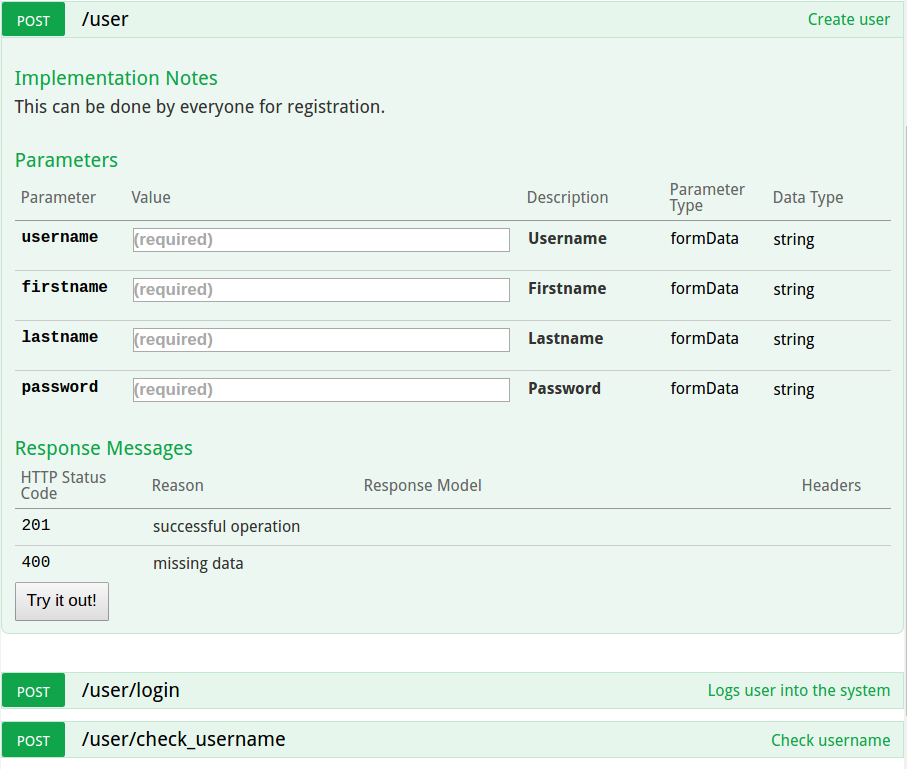
\includegraphics[width=1\textwidth]{API/user_02.png} 
\caption{Documentazione per login e registrazione}
\label{fig:user:login}
\end{figure}

\section{FUN-03}
Il terzo requisito funzionale prevede di dare la possibilità agli utenti dell'app di segnalare nuovi beacon.
Per fare ciò l'app ha bisogno di sapere dal server quali beacon sono già stati segnalati.
Troviamo quindi una rotta che ci permette di recuperare l'elenco di tutti i beacon che sono già stati segnalati senza restrizioni.

\begin{lstlisting}[caption={/webserver/app/routes/beacon.js get}, style=javaScriptCode]
  //Everybody can access to beacon list
  router.get('/', function(req, res) {
    Beacon.find({},function(err, beacons) {
      if(err) {
        res.status(500).send({msg: err.errmsg});
      } else if(beacons && beacons.length>0) {
        res.status(200).send(beacons);
      } else {
        res.status(200).send([]);
      }
    });
  });
\end{lstlisting}
Poi ha bisogno di una seconda rotta per salvare il beacon nel backend.
Questa volta, però, l'operazione potrà essere effettuata soltanto da chi ha già effettuato il login.
\begin{lstlisting}[caption={/webserver/app/routes/beacon.js aggiunta}, style=javaScriptCode]
  //User must be logged to add new beacon
  router.post('/', function(req, res) {
    if(req.user.block) {
      res.status(401).send({'msg': 'Authentication required'});
    } else if(!req.body.uuid || !req.body.major || !req.body.minor){
      res.status(400).send({'msg': 'Missing data'});
    } else {
      var newBeacon = new Beacon({
        uuid: req.body.uuid,
        major: req.body.major,
        minor: req.body.minor
      });
      newBeacon.save(function (err) {
        if(err) {
          res.status(500).send({msg: err.errmsg});
        } else {
          res.status(201).send({'msg': 'ok'});
        }
      });
    }
  });
\end{lstlisting}

Come potete osservare dalla documentazione la richiesta dei beacon è fatta in GET mentre l'aggiunta è fatta in POST.

\begin{figure}[h]
\centering
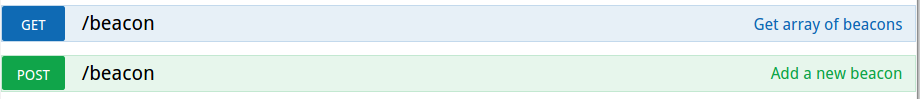
\includegraphics[width=1\textwidth]{API/beacon_03.png} 
\caption{Documentazione per login e registrazione}
\label{fig:user:login}
\end{figure}

\section{FUN-04}
Il quarto requisito prevede la possibilità di ricercare il server di Proximity System all'interno della propria LAN.

\section{FUN-05/07}
\section{FUN-08}
\section{FUN-09}
\section{FUN-10}
\section{FUN-11}
\section{FUN-12/14}